\subsection{Arquitectura}
 
 En este capítulo se presenta la arquitectura y las tecnologías involucradas en el desarrollo de la plataforma. Debido a que en los requisitos del proyecto se contempla que la plataforma quede operativa en la  DTI\footnote{Dirección de tecnologías e información} de la Universidad, el proyecto se tuvo que adaptar a la arquitectura con la que trabaja este departamento.

\subsubsection{Pseudo MVC }

El patrón de arquitectura MVC\footnote{Modelo-vista-Controlador} es una filosofía de diseño de aplicaciones que define la organización independiente del Modelo, la Vista  y el Controlador \cite{eje15}. De esta forma, el sistema se divide en tres capas donde el \textbf{modelo}  contiene una representación de los datos que maneja el sistema, es decir, el modelo de datos, la \textbf{ vista}  o interfaz de usuario contiene la información que se envía al cliente y los mecanismos de interacción con éste, y por ultimo, el \textbf{controlador} es el intermediario entre el modelo y la vista, gestionando el flujo de información entre ellos.
\\

Como se ha dicho la arquitectura MVC utiliza la división tradicional en 3 capas (presentación, lógica de negocio y datos) sin embargo la arquitectura de los proyectos de la Universidad no es específicamente  MVC, es más bien una adaptación puesto que no se separa totalmente lo que es vista del controlador, pero si se manejan de forma separada la capa de datos de la capa lógica y la interfaz de usuario, de manera semejante es como trabaja ASP.NET (se explicará en la sección \ref{ASP.NET}) . La arquitectura descrita anteriormente se detallará a continuación.
\\

	\begin{figure}[H]
		\centering
		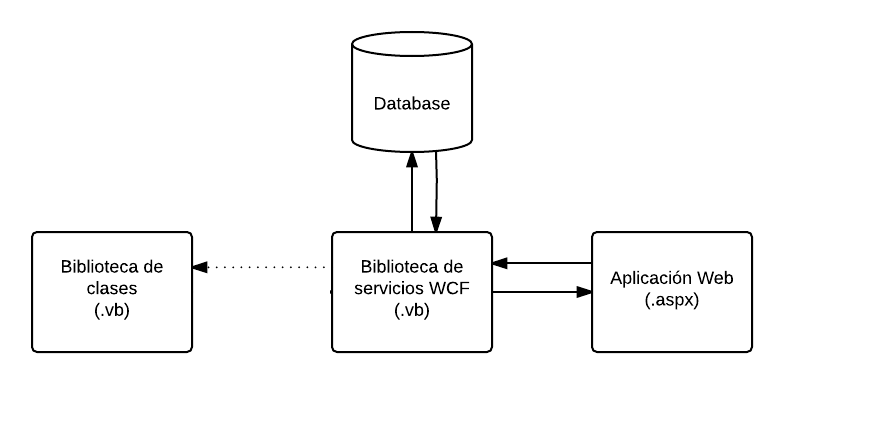
\includegraphics[width=1\textwidth]{images/Capitulo_2/pseudoMVC.png}
		\caption[Arquitectura pseudo MVC Universidad Austral de Chile]{Arquitectura pseudo MVC Universidad Austral de Chile \footnote{}}
		\label{FiguraMVC}
	\end{figure}
	\footnotetext{Elaboración propia.}
	
En la Figura \ref{FiguraMVC} se puede apreciar las 3 capas de esta arquitectua. Esta arquitectura esta compuesta por:
\begin{enumerate}
	\item \textbf{Biblioteca de servicios WCF:} Esta capa responde a eventos, usualmente acciones del usuario, e invoca los procedimientos almacenados del modelo de datos, el cual obtiene la información en la interfaz genérica de Visual Basic: IEnumerable.
	
	\item \textbf{Biblioteca de clases:} Esta capa es la encargada de darle formato a la información obtenida por la biblioteca de servicios WFC, es decir, es la representación específica de la información con la cual el sistema opera.
	
	\item \textbf{Aplicación Web:} Esta capa es la encargada de interactuar con el usuario, en ella se muestra toda la información ordenada y entendible por el usuario, sin embargo no solo posee código front-end (html, css, JavaScript, etc), si no también métodos que se comunican con los servicios WCF. Es por ello que la vista  no esta del todo separada de las reglas de negocio.
\end{enumerate}


Podemos condensar lo dicho hasta aquí, que el framework que utiliza la Universidad Austral de Chile es una forma distinta de crear aplicaciones web, si bien, se identifican claramente  la división tradicional en 3 capas (presentación, lógica de negocio y datos) no es la misma que propone el patrón MVC. En particular, en esta arquitectura  la capa \textbf{Controller} no tendría una clara correspondencia en la estructura clásica, si no que es  una mezcla de la interfaz gráfica y la lógica del negocio.

\subsection{Tecnologías para el desarrollo de la plataforma}

\subsubsection{Front-end}

Esta capa es la parte del software que interactúa con el o los usuarios, en ésta  se encuentran todas las tecnologías que corren del lado del cliente, es decir, todas aquellas tecnologías que corren del lado del navegador web. Es por ello que es de vital importancia de que el front-end sea capaz de entregar  al usuario todas las herramientas necesarias para que éste pueda realizar una correcta interacción con el sistema. Entre las tecnologías usadas en esta capa se encuentran las habituales en el desarrollo Web, tales como HTML, CSS y JavaScript junto con otras que se describirán a continuación.

\myparagraph{JQuery}

JQuery es una librería JavaScript rápida, liviana y con amplias funcionalidades. Hace mucho más simple tareas como recorrer y manipular un documento HTML, manejar eventos, animaciones, e interacciones Ajax	\footnote{Ajax: Asynchronous JavaScript And XML} por medio de una API fácil de usar que funciona a través de múltiples navegadores. Con una combinación de versatilidad y capacidad de ampliación, esta librería busca cambiar la forma en que las personas escriben JavaScript \cite{JQu15}.
\\

Si bien existen otras librerías de JavaScript (Prototype, MoonTools, entre otros). Se decidió usar JQuery en el proyecto por los siguientes motivos:
\begin{itemize}
	\item Es de uso general, por lo que posee una comunidad activa y una extensa documentación.
	\item Posee una amplia variedad de complementos que facilitan el desarrollo.
	\item Es modular.
	\item Es compatible con todos los navegadores existentes.
\end{itemize}


\myparagraph{Alertify}

Alertify es un script escrito con Jquery, el cual nos permite utilizar los siguientes elementos Javascript personalizados: alert(), confirm() y prompt(). Además también nos permite utilizar sus notificaciones, las cuales son muy agradables y sencillas de utilizar y modificar\cite{ALE15}.
\\

Alertify ha sido construido para personalizar nuestras alertas y notificaciones, de esta manera el front-end de la plataforma es mas amigable al usuario y esto permite un mejor entendimiento de los eventos que se realizan en tiempo de ejecución. Además es un plugin multi-idioma y posee responsive-design \footnote{ \textbf{ Responsive Design} es un nuevo paradigma del desarrollo web. Permite adaptar cada sitio a los diferentes formatos de dispositivos de acceso; smartphones, tabletas, portátiles, etc.}
\\

A pesar de que la mayoría de los plugins de notificaciones presentan inconvenientes al momento de implementar con vb.net, se decidió usar un sistema de alertas principalmente para facilitar la visualización de todos los eventos que ocurren en el sistema, y Alertify fue el plugin que menos problemas presentó al momento de la integración con vb.NET.


\myparagraph{Bootstrap}

Bootstrap fue creado a mediados del 2010 por un diseñador y un desarrollador de la red social Twitter, es un proyecto de código abierto, y es uno de los frameworks de front-end más populares en el mundo. Sirvió como guía de estilo para el desarrollo de herramientas internas en la empresa durante más de un año antes de su lanzamiento público, y continua haciéndolo hoy en día\cite{boo15}.
\\

El uso de un framework hace posible que el desarrollo del front-end sea: Fácil, ya que la mayoría de los framework posee una curva de aprendizaje baja, es decir, poseen una gran eficiencia en el  aprendizaje, lo que permite dominar la mayoría de los componentes en un tiempo reducido; Optimizado para dispositivos móviles, puesto que bootstrap posee todas las reglas CSS necesarias para hacer que los sitios se  adapten dinámicamente a la gran mayoría de pantallas y resoluciones existentes en el mercado.


\myparagraph{Template Metis}

Un template es un conjunto de archivos que determinan la estructura y el aspecto visual de un sitio web, y tiene como ventaja principal disminuir tiempos y costos de desarrollo \cite{gli15}. 
\\

El uso de un template disminuye el tiempo de desarrollo de un diseño web, por lo que el alumno tesista se puede centrar en la funcionalidad del sistema que es lo principal."Metis es una  template de administración gratuito basado en Twitter Bootstrap 3.x"\cite{git15}, fue diseñado por un usuario de gitHub y lo puso a disposición para que cualquier usuario lo pueda utilizar.

\myparagraph{Parsley}

 Parsley es una librería de validación de formularios, le ayuda a proporcionar a los usuarios información sobre su envío de formulario antes de enviarlo al servidor \cite{PAR15}. Fue creado por Guillaume Potier y actualmente es sustentado por Marc-André. 
\\

El uso de esta librería se sustenta en el hecho de que notificar los errores de forma inmediata  mejora la satisfacción del usuario con la aplicación y ayuda a reducir la carga de procesamiento innecesario en el servidor.

\subsubsection{Back-end}

El back-end es el área que se dedica a la parte lógica de un sitio web, es el encargado de que todo funcione como debería, el back-end no es visible para el usuario ya que no se trata de diseño, o elementos gráficos, se trata de programar las funciones que tendrá un sitio.

\myparagraph{Microsoft SQL Server 2008}

Microsoft SQL Server 2008 Express es un sistema de administración de datos eficaz y confiable que ofrece un variado conjunto de características, protección de datos y rendimiento para clientes de aplicaciones incrustadas, aplicaciones web ligeras y almacenes de datos locales \cite{mic15}.
\\



Microsoft Sql Server  esta catalogado como  una herramienta fácil de instalar, usar y administrar, por lo que muchas organizaciones hacen uso de sus servicios, tales como  Itaú, Samsung, Marcopolo, entre otras grandes compañías.
\\


Para un manejo adecuado de la base de datos se utilizará SQL Server Management Studio(SSMS), que es `` un entorno integrado para obtener acceso, configurar, administrar y desarrollar todos los componentes de SQL Server.SSMS combina un amplio grupo de herramientas gráficas con una serie de editores de script enriquecidos que permiten a desarrolladores y administradores de todos los niveles obtener acceso SQL Server" \cite{mic15}.







\myparagraph{ASP.NET} \label{ASP.NET}

ASP.NET es una plataforma web que proporciona todos los servicios necesarios para compilar aplicaciones web empresariales basadas en servidor. ASP.NET está compilado en .NET Framework, por lo que todas las características de .NET Framework están disponibles en las aplicaciones ASP.NET. Las aplicaciones se pueden escribir en cualquier lenguaje que sea compatible con Common Language Runtime (CLR), incluido Visual Basic y C\# \cite{inf15}. 
\\

ASP.NET  introduce el concepto del code-behind en el desarollo web, el cual separa el código de la interfaz de usuario, es decir,  todo lo relacionado con la Interfaz de usuario se maneja en el archivo .aspx y el control de los eventos en un archivo separado .vb (Visual Basic).Con ello se facilita la programación de aplicaciones en múltiples capas, lo que en definitiva se traduce en la total separación entre lo que el usuario ve y lo que la base de datos tiene almacenado.La ventaja del modelo  code-behind  es que no se lee secuencialmente sino que se compila, lo que incrementa de velocidad de respuesta del servidor. Además, al compilarse, el incremento en seguridad y fortaleza es muy grande. 
\\

Otro aspecto a tener en cuenta de ASP.NET es que sirve tanto para Webs sencillas como para grandes aplicaciones, ya que la orientación a objetos y la naturaleza compilada permite que la programación de sitios web sea sencilla.


\subsection{Tipos de documentos}

	
	\subsubsection{Resolución}
	\subsubsection{Comunicación interna}
	\subsubsection{Especificación de requerimientos}


